\newpage
\section{Projektowanie}		%3
%Opis przygotowania narzędzi (git, visual studio). Wybór i opis bibliotek, klas. Szkic layoutów. Pseudo kody. Opisy wykorzystanych algorytmów (np. algorytm sortowania). Dokładniejsze określenie założeń i działania aplikacji, (np.: ten przycisk otworzy takie okno a w tym oknie wpisujemy takie dane).
\subsection{Kilka słów o środowisku Android studio oraz języku programowania Java.}
\hspace{0.60cm}Android Studio to środowisko programistyczne (IDE) stworzone przez Google na bazie IntelliJ, które kierowane jest do developerów aplikacji na Androida. Pozwala ono wygodnie projektować, tworzyć i debugować własne programy na najpopularniejszą obecnie platformę systemową dla urządzeń mobilnych. Oprogramowanie oferuje podobne możliwości co środowisko Eclipse z zainstalowaną wtyczką ADT, jednak jest ono znacznie prostsze i bardziej intuicyjne w szczególności dla początkujących programistów. Przejęło ono wszystkie najlepsze rozwiązania znane użytkownikom IntelliJ, oferując narzędzie zoptymalizowane w dużym stopniu do wygodnej pracy z kodem źródłowym. Decydując się na korzystanie z Android Studio użytkownik otrzymuje środowisko programistyczne z przejrzystym i konfigurowalnym interfejsem graficznym, nie wspominając o funkcji kolorowania składni czy mechanizmie zakładek, pozwalającym na pracę z wieloma plikami jednocześnie. \newline

Java to wysokopoziomowy język programowania najczęściej wykorzystywany do tworzenia backendu aplikacji internetowych. Język ten jest łatwo przenośny, dzięki interpretowaniu przez wieloplatformową maszynę wirtualną Java Virtual Machine. Można stwierdzić, że Java jest językiem preferowanym przez korporacje i duże firmy. W Javie napisano m.in. takie aplikacje jak Gmail, OpenOffice czy Minecraft, ale także LinkedIn, Netflix czy Amazon.


\subsection{Środowisko programisty/Składanie dokumentów - Latex}
\hspace{0.60cm}Latex służy do wytwarzania przejrzyście wyglądających dokumentów tekstowych takich jak książki, artykuły, czy nawet prezentacje. Docelowym formatem jest wydruk, czy też pliki w różnych formatach, takich jak PDF, Postscript, czy też HTML. Szczególnie wygodne jest tworzenie dokumentów technicznych, matematycznych, ale z powodzeniem może też być stosowany do pisania dokumentacji programów albo zbioru opowiadań.\newline

Latex, podobnie jak języki programowania, ma swój własny język, w którym pisze się treść dokumentu oraz posiada narzędzia (można by powiedzieć "kompilatory"), które przetwarzają pliki źródłowe i generują pliki docelowe. W językach programowania zazwyczaj jedną z istotnych rzeczy jest zbiór bibliotek z gotowymi implementacjami różnych typowych czynności. Również w Latexu jest dużo gotowych pakietów pozwalających w szybki sposób tworzyć najróżniejsze elementy i rodzaje dokumentów.\newline

Filozofia Latexa jest taka, aby skupiać się na tym co merytorycznie ma zawierać dany dokument, a jak najmniej poświęcać uwagi na to, jak ma to wyglądać. Innymi słowy wprowadzamy tylko strukturę i zawartość dokumentu, a latex za nas robi resztę roboty, aby wyjściowy dokument wyglądał jak należy. Oczywiście mamy dużą możliwość ingerencji w wygląd, ale zazwyczaj jest to tylko dobieranie jakiegoś szablonu lub potrzeba uzyskania niestandardowego efektu. Jest to zupełnie inna filozofia, niż w wielu innych edytorach tekstowych, szczególnie w różnych aplikacjach biurowych, gdzie prawie na każdym kroku musimy od decydować, jaki ma być wygląd, wielkość liter, czcionka, odstępy, sposób wyświetlania tytułów itp.\newline 
Podstawą możliwości cieszenia się twórczością w Latexu jest posiadanie wszystkich narzędzi, pakietów, czcionek, itp. Gotowe zbiory są dostępne w różnych dystrybucjach. Oprócz tych narzędzi, początkujący użytkownicy mogą skorzystać z gotowych środowisk do obrabiania dokumentów Latexu.\newline
Podstawową dystrybucją jest TeX Live. Jest ona dostępna pod wiele różnych platform. Jest łatwą w instalacji kompletną paczką narzędzi, programów, czcionek.


\subsection{Czym jest Git oraz do czego służy?}
\hspace{0.60cm}Co to jest Git i dlaczego cieszy się tak dużą popularnością? Ten system kontroli wersji znacznie usprawnia, a jednocześnie zabezpiecza codzienną pracę przy kodzie. Dzięki swojej prostocie i elastyczności może być wykorzystywany zarówno przy drobnych, jak i ogromnych projektach. Dlatego też jest używany przez programistów oraz grafików na całym świecie. Odpowiadając w skrócie na pytanie, co to jest Git, należy powiedzieć, że to system kontroli wersji. Służy on więc do zarządzania historią kodu źródłowego. Jego funkcjonalność ma kilka podłoży. Między innymi sprawdza się tak dobrze, ponieważ\newline
- pozwala na jednoczesną pracę na tym samym kodzie przez kilka osób, \newline
- umożliwia transferowanie i łączenie zmian z różnych branchy w jednym projekcie\newline
- pozwala na pracę offline we własnym repozytorium \newline
- jest szybki i wydajny.\newline 
Cechy te sprawiły, że Git szybko został doceniony w całej branży. Przechowywanie wersji, a także możliwość rozgałęziania kodu to niewątpliwie jego ogromne zalety. 
\newline

GitHub z kolei to firma, która hostuje repozytoria Git i dostarcza oprogramowanie do korzystania z niego. Jednym z przykładów jest tytułowy GitHub Desktop na systemy Windows 10 i 11. GitHub jest obecnie najpopularniejszym hostem projektów open source pod względem zarówno liczby projektów , jak i użytkowników. Choć GitHub koncentruje się głównie na kodzie źródłowym, to inne projekty coraz częściej wykorzystują systemy kontrolowania wersji do zarządzania przepływem pracy związanym z publikowaniem czasopism, artykułów, podręczników itp.\newline

Test rozpoczynamy od uruchomienia naszej aplikacji a następnie pojawia nam się główne menu (rysunek 3.1), które składa się z dużych przycisków, zachowanych w kolorystyce firmy.
Na każdym z przycisków widnieje ikonka przedstawiającą daną funkcję na przykład: chcemy przetestować latarkę; klikamy przycisk, który ją przedstawia.\newline
%rysunek
\begin{figure}[!hbt]
	\begin{center}
		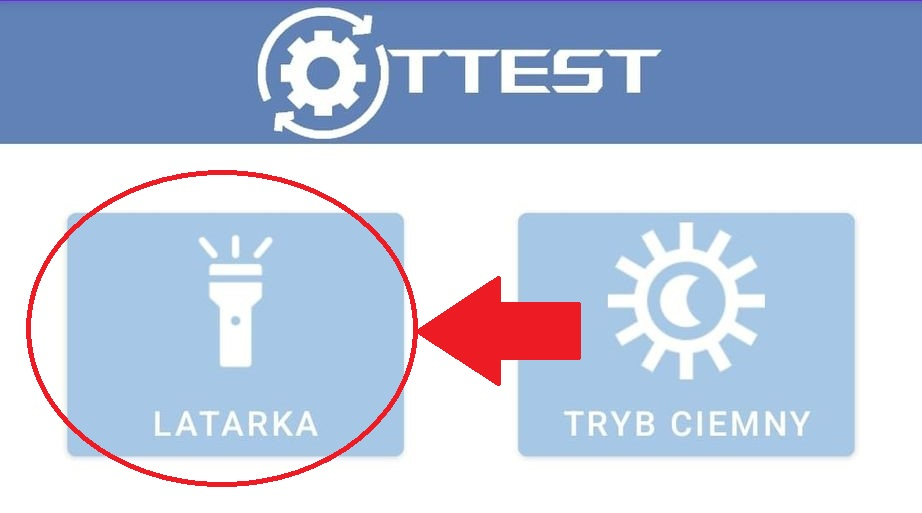
\includegraphics[angle=360, width=0.80\textwidth]{rys/przyklad_1.jpg}
		\caption{Przykładowy przycisk}
		\label{rys:przyklad}
	\end{center}
\end{figure}
\newline

Po kliknięciu ikonki, aplikacja przekierowuje nas do testu (rysunek 3.2), gdzie pojawiają się dwie latarki w centralnej części ekranu: po lewej stronie w kolorze zielonym a po prawej stronię w czerwonym. Kolor zielony ma na celu informować nas o tym że latarka jest włączona i działa, natomiast kolor czerwony sygnalizuje, że latarka jest wyłączona.
\newpage
%rysunek
\begin{figure}[!hbt]
	\begin{center}
		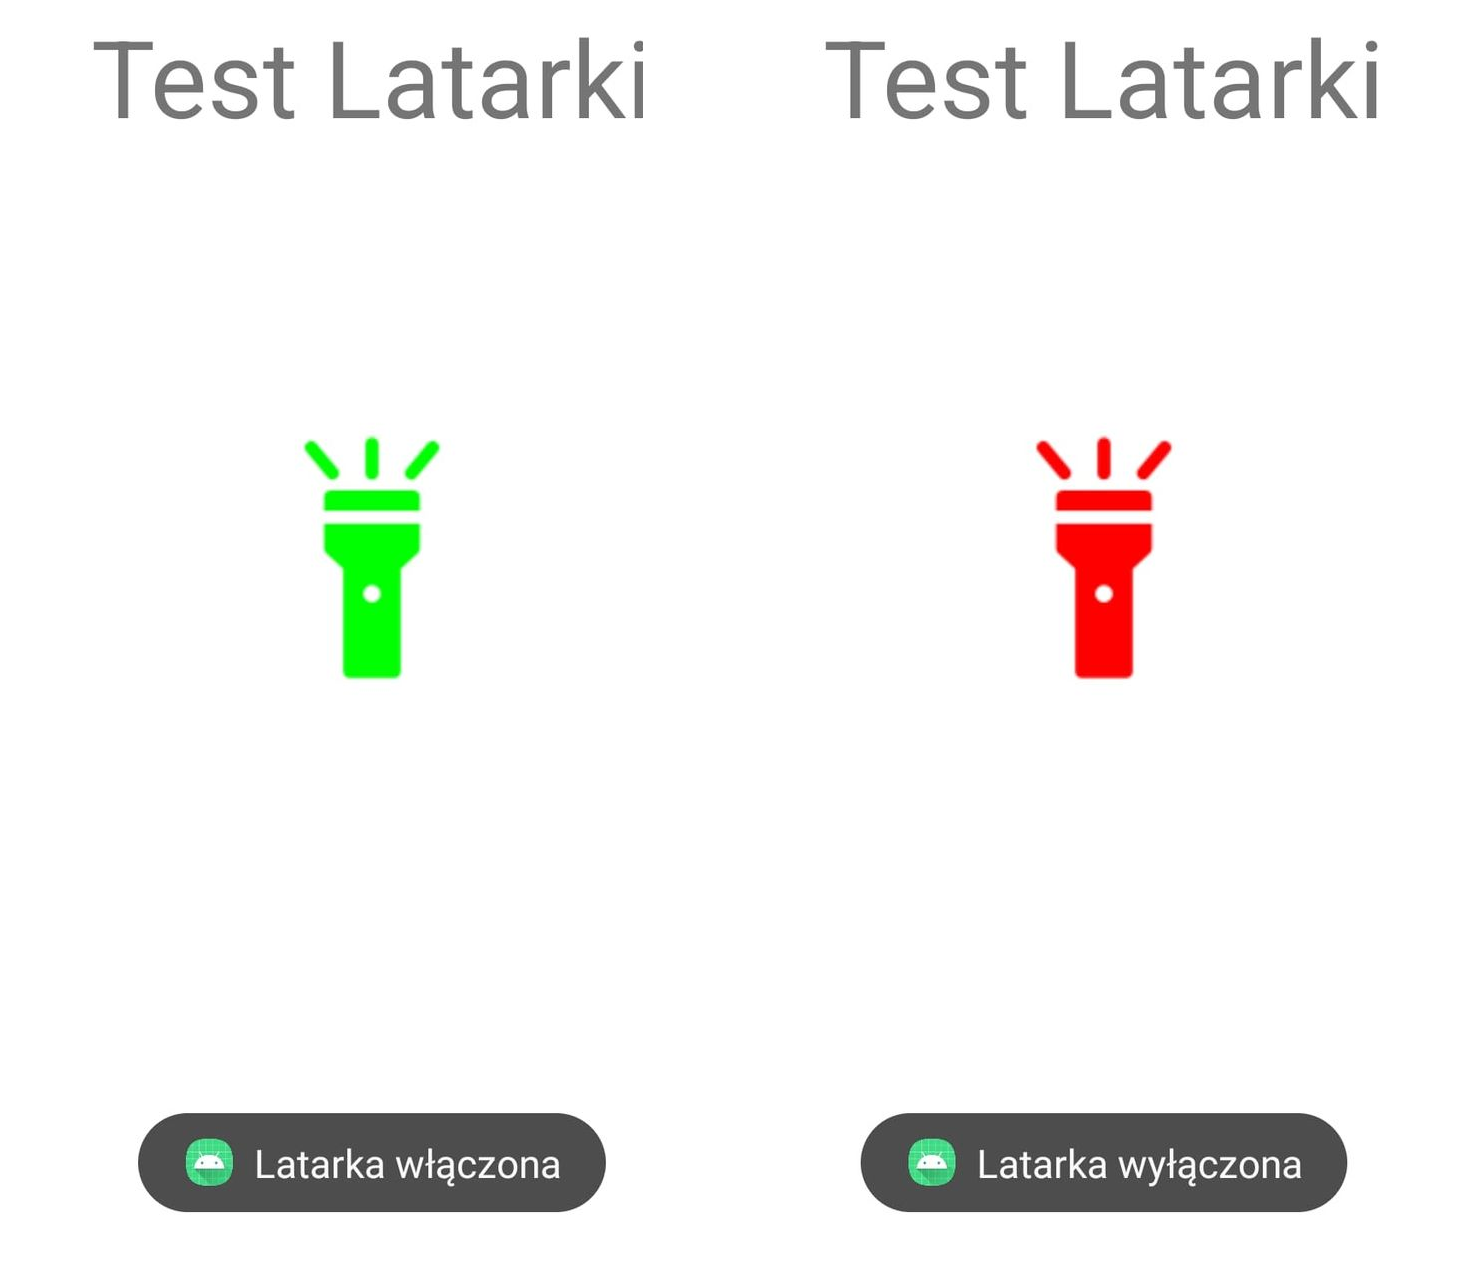
\includegraphics[angle=360, width=0.70\textwidth]{rys/przyklad_2.png}
		\caption{Test latarki}
		\label{rys:przyklad}
	\end{center}
\end{figure}   


